\documentclass{beamer}
\usepackage[utf8]{inputenc}
\usepackage[russian]{babel}
\usepackage{amsmath}
\usepackage{graphicx}
\usepackage{animate}

\title[Direction fields]{Approximation of direction fields by ODE-Net near the special points for simple ODEs}
\author{Ребриков Алексей Витальевич}
\institute{Московский физико-технический институт \\ Lab 401 \\ Курс: Прогнозирование временных рядов}
\date{3 декабря 2024 г.}

\begin{document}

\frame{\titlepage}

\begin{frame}{Цель работы}
    Построить направляющее поле и его приближение с помощью ODE-Net в окрестности особых точек для простых ОДУ (spiral, center, saddle, uniform node)
\end{frame}

\begin{frame}{Основные источники}
    \begin{itemize}
        \item [1] R. T. Q. Chen, Y. Rubanova, J. Bettencourt, D. K. Duvenaud, “Neural Ordinary Differential Equations,” \textit{Advances in Neural Information Processing Systems}, т. 32, 2019.
        \item [2] Репозиторий для библиотеки \texttt{torchdiffeq}: \url{https://github.com/rtqichen/torchdiffeq} 
    \end{itemize}
\end{frame}

\begin{frame}{О данных}
    Данные генерируются непосредственно из ОДУ:
    $$ \dot{x} = A x \quad x(0) = x_0 $$
    Отдельно train и test, начиная из разных точек
    % \includegraphics[width=\linewidth]{data_demo.png}
\end{frame}

\begin{frame}{Постановка задачи}
    Минимизировать ошибку между направляющим полем и его приближением, полученным с помощью ODE-Net.

    \vspace{1em}
    Для простоты мы просто будем минимизировать среднее значение ошибки по всем точкам.

\end{frame}

\begin{frame}{Идея ODE-Net}
    Переход от дискретного представления к <<непрерывному>> (из [1]).
    \centering
    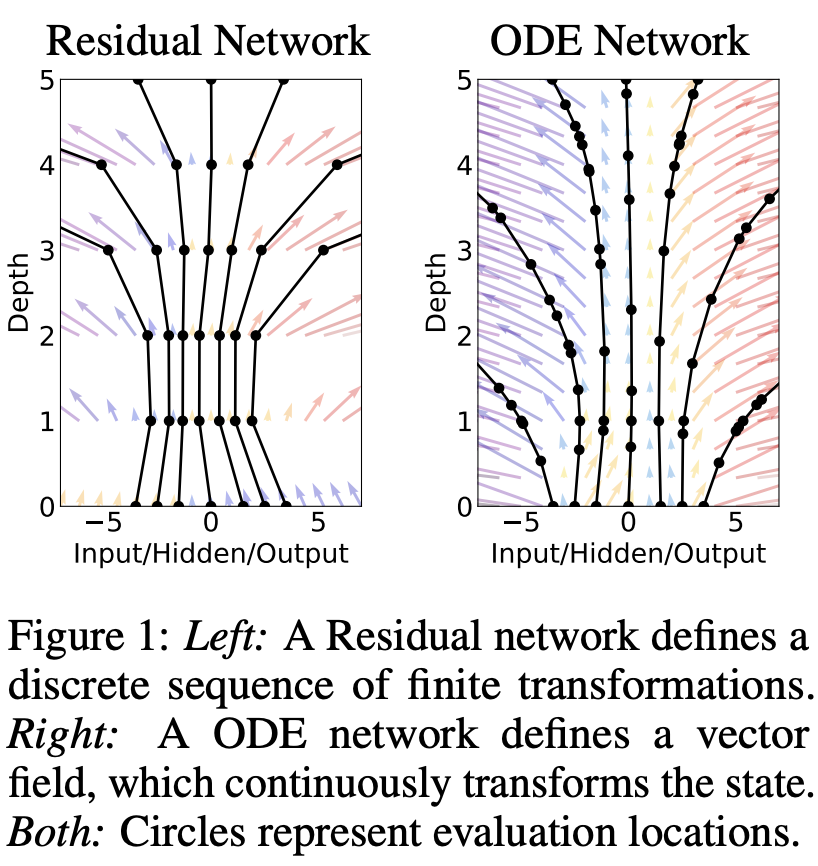
\includegraphics[width=0.6\linewidth]{../imgs/idea.png}
\end{frame}

\begin{frame}{Явный вид работы ODE-Net}
    \[
        z(t_1) = z(t_0) + \int_{t_0}^{t_1} f(z(t), t, \theta) dt = \text{ODESolve}(z(t_0), f, t_0, t_1, \theta)
    \]
    \begin{itemize}
        \item Аналогия с ResNet: \( x_{t+1} = F(x_t) + x_t \)
        \item Для нашей задачи \(f\) — линейное преобразование:
        \[
        f(z(t), t, \theta) = A(\theta) z(t)
        \]
        где \(A(\theta)\) — матрица параметров, не зависящая от \(t\).
    \end{itemize}
\end{frame}


\begin{frame}{Постановка эксперимента}
    Для каждого типа ОДУ создается соответствующая матрица \(A\) и начальные условия \(x_0\).

    Для визулизации будем использовать четыре графика:
    \begin{itemize}
        \item Явный вид траекторий одной из координат от времени (train и test)
        \item Направляющее поле и его приближение (train и test)
        \item Визуализация действия матрицы \(A\) и модели на единичную окружность
        \item Ошибка, а именно среднее значение модулей разности истинного и предсказанного направляющих полей по  точкам (train и test)
    \end{itemize}
\end{frame}

\begin{frame}{Center}
    \centering
    \animategraphics[autoplay, loop, width=\linewidth]{100}{../imgs/center-gif/frame-}{0}{24}
\end{frame}

\begin{frame}{Saddle}
    \centering
    \animategraphics[autoplay, loop, width=\linewidth]{100}{../imgs/saddle-gif/frame-}{0}{24}
\end{frame}

\begin{frame}{Spiral}
    \centering
    \animategraphics[autoplay, loop, width=\linewidth]{100}{../imgs/spiral-gif/frame-}{0}{24}
\end{frame}

\begin{frame}{Uniform node}
    \centering
    \animategraphics[autoplay, loop, width=\linewidth]{100}{../imgs/uniform-gif/frame-}{0}{24}
\end{frame}

\begin{frame}{Выводы}
    \begin{itemize}
        \item Для простых ОДУ ODE-Net работает достаточно хорошо, особенно для center и spiral.
        \item Для saddle чуть хуже, но тоже неплохо
        \item Для uniform node не смог восстановить направляющее поле, все дело в том что только одно направление было правильно предсказано, а по втором масштаб никак не понять.
    \end{itemize}
\end{frame}

\begin{frame}{Будущие работы}
    \begin{itemize}
        \item Попробовать запускать не из одной начальной точки, а нескольких (должно починить проблему с uniform node и узлом)
        \item Попробовать для более сложных ОДУ
    \end{itemize}
\end{frame}

\end{document}

